% Options for packages loaded elsewhere
\PassOptionsToPackage{unicode}{hyperref}
\PassOptionsToPackage{hyphens}{url}
%
\documentclass[
]{article}
\usepackage{amsmath,amssymb}
\usepackage{lmodern}
\usepackage{ifxetex,ifluatex}
\ifnum 0\ifxetex 1\fi\ifluatex 1\fi=0 % if pdftex
  \usepackage[T1]{fontenc}
  \usepackage[utf8]{inputenc}
  \usepackage{textcomp} % provide euro and other symbols
\else % if luatex or xetex
  \usepackage{unicode-math}
  \defaultfontfeatures{Scale=MatchLowercase}
  \defaultfontfeatures[\rmfamily]{Ligatures=TeX,Scale=1}
\fi
% Use upquote if available, for straight quotes in verbatim environments
\IfFileExists{upquote.sty}{\usepackage{upquote}}{}
\IfFileExists{microtype.sty}{% use microtype if available
  \usepackage[]{microtype}
  \UseMicrotypeSet[protrusion]{basicmath} % disable protrusion for tt fonts
}{}
\makeatletter
\@ifundefined{KOMAClassName}{% if non-KOMA class
  \IfFileExists{parskip.sty}{%
    \usepackage{parskip}
  }{% else
    \setlength{\parindent}{0pt}
    \setlength{\parskip}{6pt plus 2pt minus 1pt}}
}{% if KOMA class
  \KOMAoptions{parskip=half}}
\makeatother
\usepackage{xcolor}
\IfFileExists{xurl.sty}{\usepackage{xurl}}{} % add URL line breaks if available
\IfFileExists{bookmark.sty}{\usepackage{bookmark}}{\usepackage{hyperref}}
\hypersetup{
  pdftitle={Mapping scientific communities at scale},
  pdfkeywords={French publications, Machine
learning, scanR, OpenAlex, Biblioglutton, Elasticsearch},
  hidelinks,
  pdfcreator={LaTeX via pandoc}}
\urlstyle{same} % disable monospaced font for URLs
\usepackage[left=3cm, right=3cm, top=3cm, bottom=3cm]{geometry}
\usepackage{color}
\usepackage{fancyvrb}
\newcommand{\VerbBar}{|}
\newcommand{\VERB}{\Verb[commandchars=\\\{\}]}
\DefineVerbatimEnvironment{Highlighting}{Verbatim}{commandchars=\\\{\}}
% Add ',fontsize=\small' for more characters per line
\newenvironment{Shaded}{}{}
\newcommand{\AlertTok}[1]{\textcolor[rgb]{1.00,0.00,0.00}{\textbf{#1}}}
\newcommand{\AnnotationTok}[1]{\textcolor[rgb]{0.38,0.63,0.69}{\textbf{\textit{#1}}}}
\newcommand{\AttributeTok}[1]{\textcolor[rgb]{0.49,0.56,0.16}{#1}}
\newcommand{\BaseNTok}[1]{\textcolor[rgb]{0.25,0.63,0.44}{#1}}
\newcommand{\BuiltInTok}[1]{#1}
\newcommand{\CharTok}[1]{\textcolor[rgb]{0.25,0.44,0.63}{#1}}
\newcommand{\CommentTok}[1]{\textcolor[rgb]{0.38,0.63,0.69}{\textit{#1}}}
\newcommand{\CommentVarTok}[1]{\textcolor[rgb]{0.38,0.63,0.69}{\textbf{\textit{#1}}}}
\newcommand{\ConstantTok}[1]{\textcolor[rgb]{0.53,0.00,0.00}{#1}}
\newcommand{\ControlFlowTok}[1]{\textcolor[rgb]{0.00,0.44,0.13}{\textbf{#1}}}
\newcommand{\DataTypeTok}[1]{\textcolor[rgb]{0.56,0.13,0.00}{#1}}
\newcommand{\DecValTok}[1]{\textcolor[rgb]{0.25,0.63,0.44}{#1}}
\newcommand{\DocumentationTok}[1]{\textcolor[rgb]{0.73,0.13,0.13}{\textit{#1}}}
\newcommand{\ErrorTok}[1]{\textcolor[rgb]{1.00,0.00,0.00}{\textbf{#1}}}
\newcommand{\ExtensionTok}[1]{#1}
\newcommand{\FloatTok}[1]{\textcolor[rgb]{0.25,0.63,0.44}{#1}}
\newcommand{\FunctionTok}[1]{\textcolor[rgb]{0.02,0.16,0.49}{#1}}
\newcommand{\ImportTok}[1]{#1}
\newcommand{\InformationTok}[1]{\textcolor[rgb]{0.38,0.63,0.69}{\textbf{\textit{#1}}}}
\newcommand{\KeywordTok}[1]{\textcolor[rgb]{0.00,0.44,0.13}{\textbf{#1}}}
\newcommand{\NormalTok}[1]{#1}
\newcommand{\OperatorTok}[1]{\textcolor[rgb]{0.40,0.40,0.40}{#1}}
\newcommand{\OtherTok}[1]{\textcolor[rgb]{0.00,0.44,0.13}{#1}}
\newcommand{\PreprocessorTok}[1]{\textcolor[rgb]{0.74,0.48,0.00}{#1}}
\newcommand{\RegionMarkerTok}[1]{#1}
\newcommand{\SpecialCharTok}[1]{\textcolor[rgb]{0.25,0.44,0.63}{#1}}
\newcommand{\SpecialStringTok}[1]{\textcolor[rgb]{0.73,0.40,0.53}{#1}}
\newcommand{\StringTok}[1]{\textcolor[rgb]{0.25,0.44,0.63}{#1}}
\newcommand{\VariableTok}[1]{\textcolor[rgb]{0.10,0.09,0.49}{#1}}
\newcommand{\VerbatimStringTok}[1]{\textcolor[rgb]{0.25,0.44,0.63}{#1}}
\newcommand{\WarningTok}[1]{\textcolor[rgb]{0.38,0.63,0.69}{\textbf{\textit{#1}}}}
\usepackage{graphicx}
\makeatletter
\def\maxwidth{\ifdim\Gin@nat@width>\linewidth\linewidth\else\Gin@nat@width\fi}
\def\maxheight{\ifdim\Gin@nat@height>\textheight\textheight\else\Gin@nat@height\fi}
\makeatother
% Scale images if necessary, so that they will not overflow the page
% margins by default, and it is still possible to overwrite the defaults
% using explicit options in \includegraphics[width, height, ...]{}
\setkeys{Gin}{width=\maxwidth,height=\maxheight,keepaspectratio}
% Set default figure placement to htbp
\makeatletter
\def\fps@figure{htbp}
\makeatother
\setlength{\emergencystretch}{3em} % prevent overfull lines
\providecommand{\tightlist}{%
  \setlength{\itemsep}{0pt}\setlength{\parskip}{0pt}}
\setcounter{secnumdepth}{-\maxdimen} % remove section numbering
\ifluatex
  \usepackage{selnolig}  % disable illegal ligatures
\fi
\newlength{\cslhangindent}
\setlength{\cslhangindent}{1.5em}
\newlength{\csllabelwidth}
\setlength{\csllabelwidth}{3em}
\newenvironment{CSLReferences}[2] % #1 hanging-ident, #2 entry spacing
 {% don't indent paragraphs
  \setlength{\parindent}{0pt}
  % turn on hanging indent if param 1 is 1
  \ifodd #1 \everypar{\setlength{\hangindent}{\cslhangindent}}\ignorespaces\fi
  % set entry spacing
  \ifnum #2 > 0
  \setlength{\parskip}{#2\baselineskip}
  \fi
 }%
 {}
\usepackage{calc}
\newcommand{\CSLBlock}[1]{#1\hfill\break}
\newcommand{\CSLLeftMargin}[1]{\parbox[t]{\csllabelwidth}{#1}}
\newcommand{\CSLRightInline}[1]{\parbox[t]{\linewidth - \csllabelwidth}{#1}\break}
\newcommand{\CSLIndent}[1]{\hspace{\cslhangindent}#1}
% for compatibility with pandoc 2.10
\newenvironment{cslreferences}%
  {\setlength{\parindent}{0pt}%
  \everypar{\setlength{\hangindent}{\cslhangindent}}\ignorespaces}%
  {\par}

\title{Mapping scientific communities at scale}
\usepackage{authblk}
\author[%
  1%
  ]{%
  Hafsa Aallat%
  %
  %
}
\affil[1]{French Ministry of Higher Education and Research, Paris,
France}
\date{February 2025}

\makeatletter
\def\@maketitle{%
  \newpage \null \vskip 2em
  \begin {center}%
    \let \footnote \thanks
         {\LARGE \@title \par}%
         \vskip 1.5em%
                {\large \lineskip .5em%
                  \begin {tabular}[t]{c}%
                    \@author
                  \end {tabular}\par}%
                                                \vskip 1em{\large \@date}%
  \end {center}%
  \par
  \vskip 1.5em}
\makeatother

\begin{document}
\maketitle

\textbf{Keywords}: french publications, machine learning, open data,
open source

\hypertarget{motivation}{%
\section{1. Motivation}\label{motivation}}

\hypertarget{presentation-of-ipcc-and-ipbes-working-groups-and-dates}{%
\subsection{1.1 Presentation of IPCC and IPBES: Working Groups and
dates}\label{presentation-of-ipcc-and-ipbes-working-groups-and-dates}}

\textbf{The IPCC (Intergovernmental Panel on Climate Change)} assesses
scientific information on climate change, providing reports to guide
policymakers. It has three working groups sees as three main themes :

\begin{itemize}
\tightlist
\item
  Working Group I (WGI) focuses on the \textbf{physical science} of
  climate change.
\item
  Working Group II (WGII) examines climate change impacts,
  \textbf{adaptation}, and vulnerabilities.
\item
  Working Group III (WGIII) addresses climate change \textbf{mitigation}
  strategies.
\end{itemize}

The Sixth Assessment Report (AR6) was released in stages between 2021
and 2022.

\textbf{The IPBES (Intergovernmental Science-Policy Platform on
Biodiversity and Ecosystem Services)}, established in 2012, assesses
biodiversity and ecosystem services. It produces thematic and regional
assessments, with the \textbf{Global Assessment Report (2019)}
highlighting biodiversity loss and the need for urgent action.

Both platforms provide crucial scientific assessments that inform global
climate and biodiversity policies.

\hypertarget{limits-of-the-french-court-of-audit-study}{%
\subsection{1.2 Limits of the French Court of Audit
study}\label{limits-of-the-french-court-of-audit-study}}

In 2023, the French Court of Audit conducted a study on France's
scientific output related to environmental transition. After hearings
with the Directorate General for Research and Innovation (DGRI) and
research operators, the Court analyzed the bibliography cited in the
sixth IPCC report. The study found that French publications are the most
cited in the physical sciences of climate change, highlighting the
global impact of French research in this field.

However, this evaluation has important limitations. The IPCC
bibliography is based on high-impact publications often from top
journals, making it quite selective. This selection prioritizes more
visible and well-known works, leaving out other important research that
may not be as visible but still in the same themes as IPCC report. While
this reflects France's scientific excellence, it does not fully
represent the diversity of French scientific contributions to ecological
transition.

\hypertarget{how-can-we-explore-and-recognize-french-publications-related-to-the-same-topics-as-ipcc-report-from-a-global-point-of-view}{%
\subsection{1.3 How can we explore and recognize french publications
related to the same topics as IPCC report from a global point of view
?}\label{how-can-we-explore-and-recognize-french-publications-related-to-the-same-topics-as-ipcc-report-from-a-global-point-of-view}}

To fill this gap, we propose using a larger dataset, such as scanR.
\textbf{ScanR has a significantly higher coverage} of publications with
at least one French affiliation compared to other sources, contributing
92\% to the overall aggregated corpus. This is much higher than
databases like Scopus (67\%), WoS (58\%), or PubMed (29\%), making ScanR
a more comprehensive tool for capturing French scientific publications
(Chaignon and Egret 2022). Unlike the IPCC's restricted approach, ScanR
includes publications with at least one French affiliation, showing a
larger view of research. This could allow us to capture a more diverse
range of topics related to climate change physical science, adaptation
and mitigation.

Initially, we will replicate the Court of Audit analysis of the IPCC
bibliography to identify the main themes and their proportion of French
contributions. Then, we will expand our study to know the top
institutions, labs, regions, and researchers that provide solutions to
the challenges of environemental transition in France, based on IPCC
bibliography. In a second time, we will create a model that can
recognize a publication about IPCC similar topics, and apply the model
to scanR publications. At the same time, we will conduct a similar
analysis for the IPBES bibliography, following the same approach to
identify the French contributions, and exploring less visible but
valuable research related to biodiversity and ecosystem services.

\hypertarget{ipcc-and-ipbes-bibliography-analysis-and-model}{%
\section{2. IPCC and IPBES Bibliography Analysis and
Model}\label{ipcc-and-ipbes-bibliography-analysis-and-model}}

We propose a method to analyze the bibliographies of IPCC and IPBES
reports.

\hypertarget{data-collection-and-cleaning}{%
\subsection{2.1 Data Collection and
Cleaning}\label{data-collection-and-cleaning}}

For each report, we collect the references:

\begin{itemize}
\tightlist
\item
  For IPCC report, we collect citations in .bib format for each chapter
  of each working group (n.d.a).
\item
  For IPBES report, we gather all citations via Zotero (n.d.b).
\end{itemize}

Once the data is collected, we clean the DOI (Digital Object Identifier)
of each publication. The DOI should follow a specific format starting
with `10.'. Any publication without a valid DOI is not considered.

\hypertarget{data-enrichment}{%
\subsection{2.2 Data Enrichment}\label{data-enrichment}}

After cleaning, the data contains features such as DOI, title, and main
author. However, we still lack information such as institutions,
researchers, countries, and topics associated with each publication. To
fill in the gap, we enrich the data by importing additional features
from OpenAlex for each publication with a valid DOI. These features
include: countries, year, topics, title, author names, institutions,
RORs (Research Organization Registry) and journals.

OpenAlex is an international open-access database that provides metadata
on research papers, authors, journals, and institutions. It aims to make
academic information more accessible and supports data analysis and
knowledge discovery in various fields. OpenAlex is a valuable tool for
researchers and educators. We use the Api to import the features.

Next, we use the Biblioglutton Python library to fill in missing DOIs
based on the title and main author. We also verify that the year
retrieved from OpenAlex matches the year in the original dataset.

\hypertarget{data-storage-and-visualization}{%
\subsection{2.3 Data storage and
visualization}\label{data-storage-and-visualization}}

Once the data is enriched with openAlex features, we edit the data and
push them on a cluster elastic-search. As an exemple, for one
publication (for a better visibility the data is troncated). Some
publications are used by both reports, with the following keys:

\begin{Shaded}
\begin{Highlighting}[]
\FunctionTok{\{}
  \DataTypeTok{"doi"}\FunctionTok{:} \StringTok{"10.1126/science.aaw6974"}\FunctionTok{,}
  \DataTypeTok{"year"}\FunctionTok{:} \StringTok{"2018"}\FunctionTok{,}
  \DataTypeTok{"title"}\FunctionTok{:} \StringTok{"Impacts of 1.5 °C global warming on natural and human systems"}\FunctionTok{,}
  \DataTypeTok{"rors"}\FunctionTok{:} \OtherTok{[}
    \OtherTok{[}\StringTok{"https://ror.org/00rqy9422"}\OtherTok{,} \StringTok{"AU"}\OtherTok{],}
    \OtherTok{[}\StringTok{"https://ror.org/03ztgj037"}\OtherTok{,} \StringTok{"DE"}\OtherTok{],}
    \OtherTok{[}\StringTok{"https://ror.org/05sbt2524"}\OtherTok{,} \StringTok{"FR"}\OtherTok{],}
    \OtherTok{[}\StringTok{"..."}\OtherTok{]}
  \OtherTok{]}\FunctionTok{,}
  \DataTypeTok{"ipcc"}\FunctionTok{:} \OtherTok{[}
    \FunctionTok{\{} \DataTypeTok{"name"}\FunctionTok{:} \StringTok{"wg1\_chap\_01"}\FunctionTok{,} \DataTypeTok{"wg"}\FunctionTok{:} \StringTok{"1"}\FunctionTok{,} \DataTypeTok{"chap"}\FunctionTok{:} \DecValTok{1} \FunctionTok{\}}\OtherTok{,}
    \FunctionTok{\{} \DataTypeTok{"name"}\FunctionTok{:} \StringTok{"wg2\_chap\_01"}\FunctionTok{,} \DataTypeTok{"wg"}\FunctionTok{:} \StringTok{"2"}\FunctionTok{,} \DataTypeTok{"chap"}\FunctionTok{:} \DecValTok{1} \FunctionTok{\}}\OtherTok{,}
    \FunctionTok{\{} \DataTypeTok{"name"}\FunctionTok{:} \StringTok{"wg2\_chap\_02"}\FunctionTok{,} \DataTypeTok{"wg"}\FunctionTok{:} \StringTok{"2"}\FunctionTok{,} \DataTypeTok{"chap"}\FunctionTok{:} \DecValTok{2} \FunctionTok{\}}\OtherTok{,}
    \FunctionTok{\{} \DataTypeTok{"name"}\FunctionTok{:} \StringTok{"wg2\_chap\_04"}\FunctionTok{,} \DataTypeTok{"wg"}\FunctionTok{:} \StringTok{"2"}\FunctionTok{,} \DataTypeTok{"chap"}\FunctionTok{:} \DecValTok{4} \FunctionTok{\}}\OtherTok{,}
    \FunctionTok{\{} \DataTypeTok{"name"}\FunctionTok{:} \StringTok{"wg2\_chap\_07"}\FunctionTok{,} \DataTypeTok{"wg"}\FunctionTok{:} \StringTok{"2"}\FunctionTok{,} \DataTypeTok{"chap"}\FunctionTok{:} \DecValTok{7} \FunctionTok{\}}\OtherTok{,}
    \FunctionTok{\{} \DataTypeTok{"name"}\FunctionTok{:} \StringTok{"wg2\_chap\_08"}\FunctionTok{,} \DataTypeTok{"wg"}\FunctionTok{:} \StringTok{"2"}\FunctionTok{,} \DataTypeTok{"chap"}\FunctionTok{:} \DecValTok{8} \FunctionTok{\}}\OtherTok{,}
    \FunctionTok{\{} \DataTypeTok{"name"}\FunctionTok{:} \StringTok{"wg2\_chap\_12"}\FunctionTok{,} \DataTypeTok{"wg"}\FunctionTok{:} \StringTok{"2"}\FunctionTok{,} \DataTypeTok{"chap"}\FunctionTok{:} \DecValTok{12} \FunctionTok{\}}\OtherTok{,}
    \FunctionTok{\{} \DataTypeTok{"name"}\FunctionTok{:} \StringTok{"wg2\_chap\_13"}\FunctionTok{,} \DataTypeTok{"wg"}\FunctionTok{:} \StringTok{"2"}\FunctionTok{,} \DataTypeTok{"chap"}\FunctionTok{:} \DecValTok{13} \FunctionTok{\}}\OtherTok{,}
    \FunctionTok{\{} \DataTypeTok{"name"}\FunctionTok{:} \StringTok{"wg2\_chap\_14"}\FunctionTok{,} \DataTypeTok{"wg"}\FunctionTok{:} \StringTok{"2"}\FunctionTok{,} \DataTypeTok{"chap"}\FunctionTok{:} \DecValTok{14} \FunctionTok{\}}\OtherTok{,}
    \FunctionTok{\{} \DataTypeTok{"name"}\FunctionTok{:} \StringTok{"wg2\_chap\_15"}\FunctionTok{,} \DataTypeTok{"wg"}\FunctionTok{:} \StringTok{"2"}\FunctionTok{,} \DataTypeTok{"chap"}\FunctionTok{:} \DecValTok{15} \FunctionTok{\}}\OtherTok{,}
    \FunctionTok{\{} \DataTypeTok{"name"}\FunctionTok{:} \StringTok{"wg2\_chap\_16"}\FunctionTok{,} \DataTypeTok{"wg"}\FunctionTok{:} \StringTok{"2"}\FunctionTok{,} \DataTypeTok{"chap"}\FunctionTok{:} \DecValTok{16} \FunctionTok{\}}\OtherTok{,}
    \FunctionTok{\{} \DataTypeTok{"name"}\FunctionTok{:} \StringTok{"wg2\_cross\_chap\_1"}\FunctionTok{,} \DataTypeTok{"wg"}\FunctionTok{:} \StringTok{"2\_cross"}\FunctionTok{,} \DataTypeTok{"chap"}\FunctionTok{:} \DecValTok{1} \FunctionTok{\}}\OtherTok{,}
    \FunctionTok{\{} \DataTypeTok{"name"}\FunctionTok{:} \StringTok{"wg2\_cross\_chap\_4"}\FunctionTok{,} \DataTypeTok{"wg"}\FunctionTok{:} \StringTok{"2\_cross"}\FunctionTok{,} \DataTypeTok{"chap"}\FunctionTok{:} \DecValTok{4} \FunctionTok{\}}\OtherTok{,}
    \FunctionTok{\{} \DataTypeTok{"name"}\FunctionTok{:} \StringTok{"wg3\_chap\_01"}\FunctionTok{,} \DataTypeTok{"wg"}\FunctionTok{:} \StringTok{"3"}\FunctionTok{,} \DataTypeTok{"chap"}\FunctionTok{:} \DecValTok{1} \FunctionTok{\}}\OtherTok{,}
    \FunctionTok{\{} \DataTypeTok{"name"}\FunctionTok{:} \StringTok{"wg3\_chap\_04"}\FunctionTok{,} \DataTypeTok{"wg"}\FunctionTok{:} \StringTok{"3"}\FunctionTok{,} \DataTypeTok{"chap"}\FunctionTok{:} \DecValTok{4} \FunctionTok{\}}
  \OtherTok{]}\FunctionTok{,}
  \DataTypeTok{"authors\_name"}\FunctionTok{:} \OtherTok{[}
    \OtherTok{[}\StringTok{"Ove Hoegh‐Guldberg"}\OtherTok{,} \OtherTok{[}\StringTok{"AU"}\OtherTok{]],}
    \OtherTok{[}\StringTok{"Daniela Jacob"}\OtherTok{,} \OtherTok{[}\StringTok{"DE"}\OtherTok{]],}
    \OtherTok{[}\StringTok{"Michael A. Taylor"}\OtherTok{,} \OtherTok{[}\StringTok{"JM"}\OtherTok{]],}
    \OtherTok{[}\StringTok{"..."}\OtherTok{]}
  \OtherTok{]}\FunctionTok{,}
  \DataTypeTok{"institutions\_names"}\FunctionTok{:} \OtherTok{[}
    \OtherTok{[}\StringTok{"University of Queensland"}\OtherTok{,} \StringTok{"AU"}\OtherTok{],}
    \OtherTok{[}\StringTok{"German Climate Computing Centre"}\OtherTok{,} \StringTok{"DE"}\OtherTok{],}
    \OtherTok{[}\StringTok{"University of the West Indies"}\OtherTok{,} \StringTok{"JM"}\OtherTok{],}
    \OtherTok{[}\StringTok{"..."}\OtherTok{]}
  \OtherTok{]}\FunctionTok{,}
  \DataTypeTok{"countries"}\FunctionTok{:} \OtherTok{[}\StringTok{"CHN"}\OtherTok{,} \StringTok{"GBR"}\OtherTok{,} \StringTok{"FRA"}\OtherTok{,} \StringTok{"..."}\OtherTok{]}\FunctionTok{,}
  \DataTypeTok{"ipbes"}\FunctionTok{:} \OtherTok{[}\FunctionTok{\{} \DataTypeTok{"chapter"}\FunctionTok{:} \StringTok{"4"} \FunctionTok{\}}\OtherTok{]}\FunctionTok{,}
  \DataTypeTok{"topics"}\FunctionTok{:} \OtherTok{[}
    \StringTok{"Impact of Climate Change on Human Migration"}\OtherTok{,}
    \StringTok{"Geoengineering and Climate Ethics"}\OtherTok{,}
    \StringTok{"Economic Implications of Climate Change Policies"}
  \OtherTok{]}
\FunctionTok{\}}
\end{Highlighting}
\end{Shaded}

After that we used Highcharts, a graphic tool to visualize the graphs.
At the same time, we plot the graphs also with python by making
elastic-search requests.

\hypertarget{create-a-database}{%
\subsection{2.4 Create a database}\label{create-a-database}}

In the enriched database derived from the IPCC and IPBES publications,
each publication is associated with the following attributes:

\begin{itemize}
\tightlist
\item
  A unique identifier (\textbf{DOI})
\item
  The publication \textbf{year}
\item
  A \textbf{title} that best summarizes the publication
\item
  The \textbf{main themes} covered by the publication
\item
  The names of the \textbf{journals} in which the publication was
  published
\end{itemize}

Out of the 53,258 IPCC publications available on OpenAlex, only 48,219
have non-empty titles, themes, and journal names.

The goal is to identify these 48,219 publications that are not cited by
the IPCC to form our training dataset.

After the analysis phase, we were wondering how to make a database with
data from IPCC bibliography and data from other subjects than IPCC
topics.

Initially, we explore the data from the reports and analize:

\begin{itemize}
\tightlist
\item
  Their temporal distribution
\item
  The main topics
\item
  The main journals were the publications are released
\end{itemize}

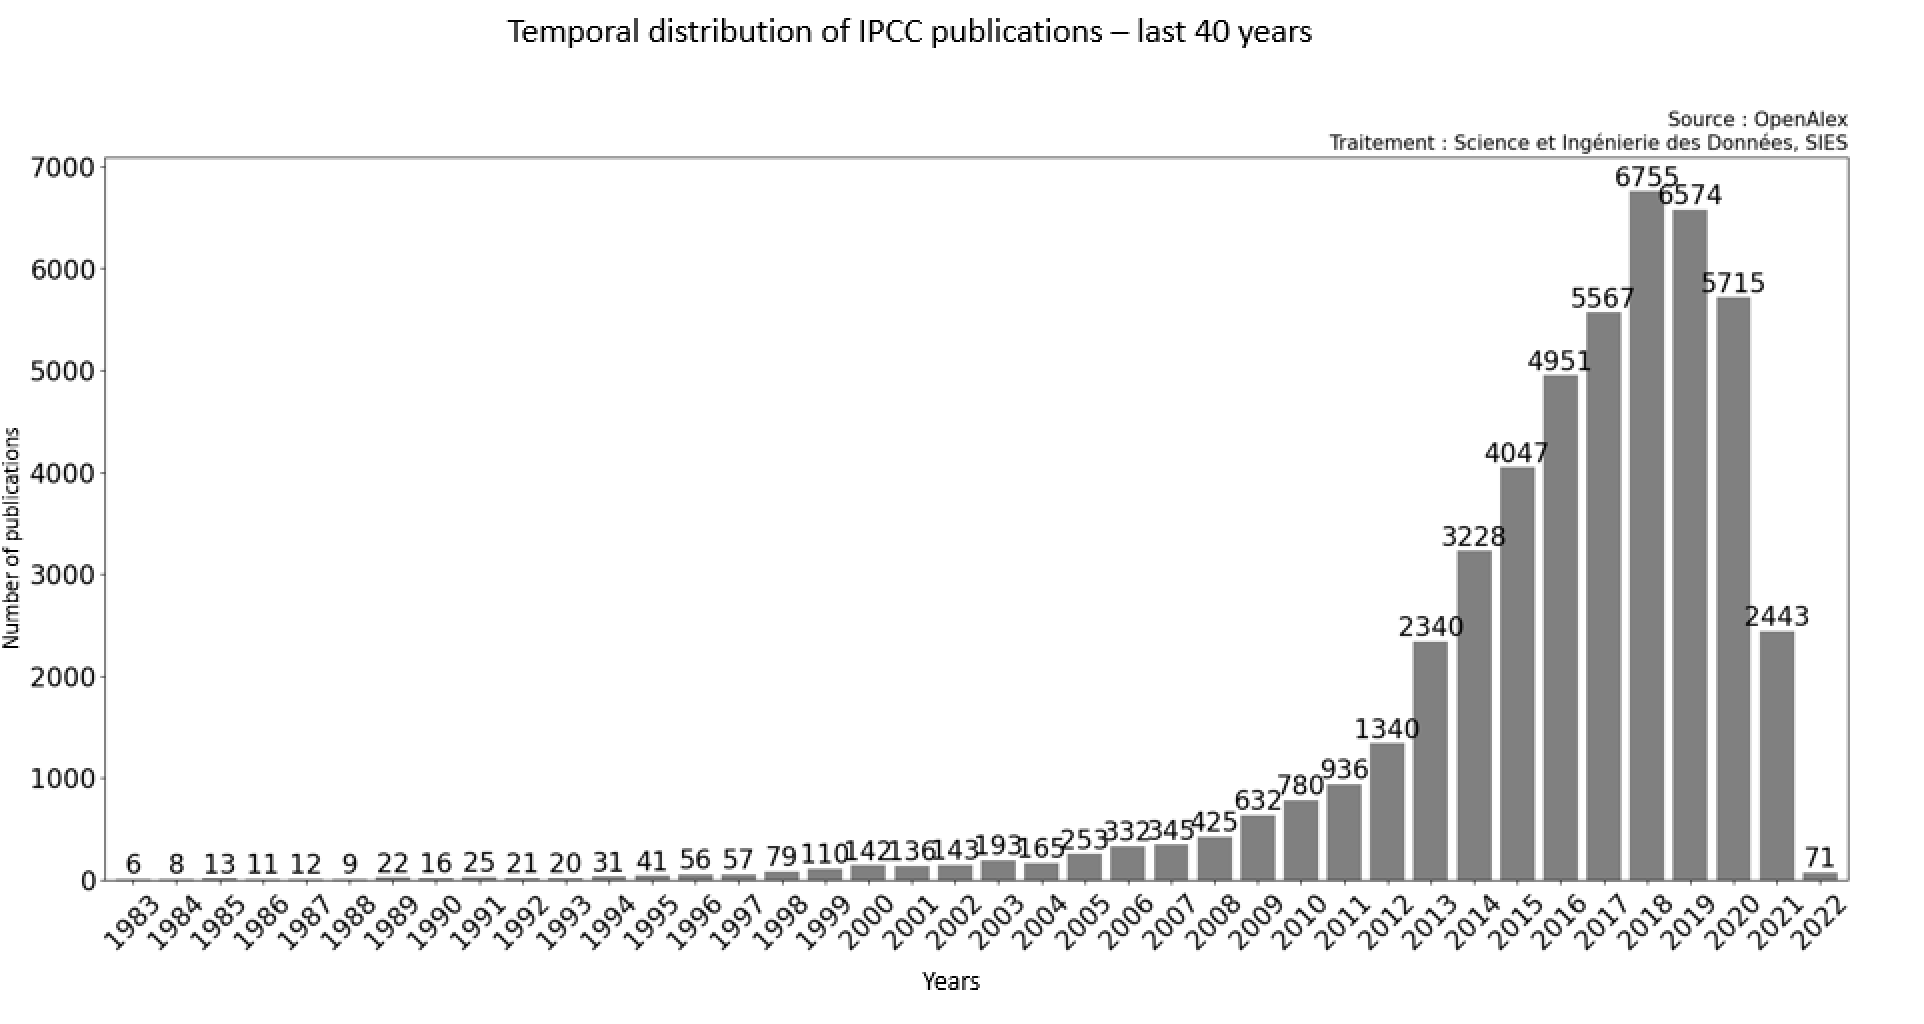
\includegraphics{./images/time_distribution_IPCC_model.png}
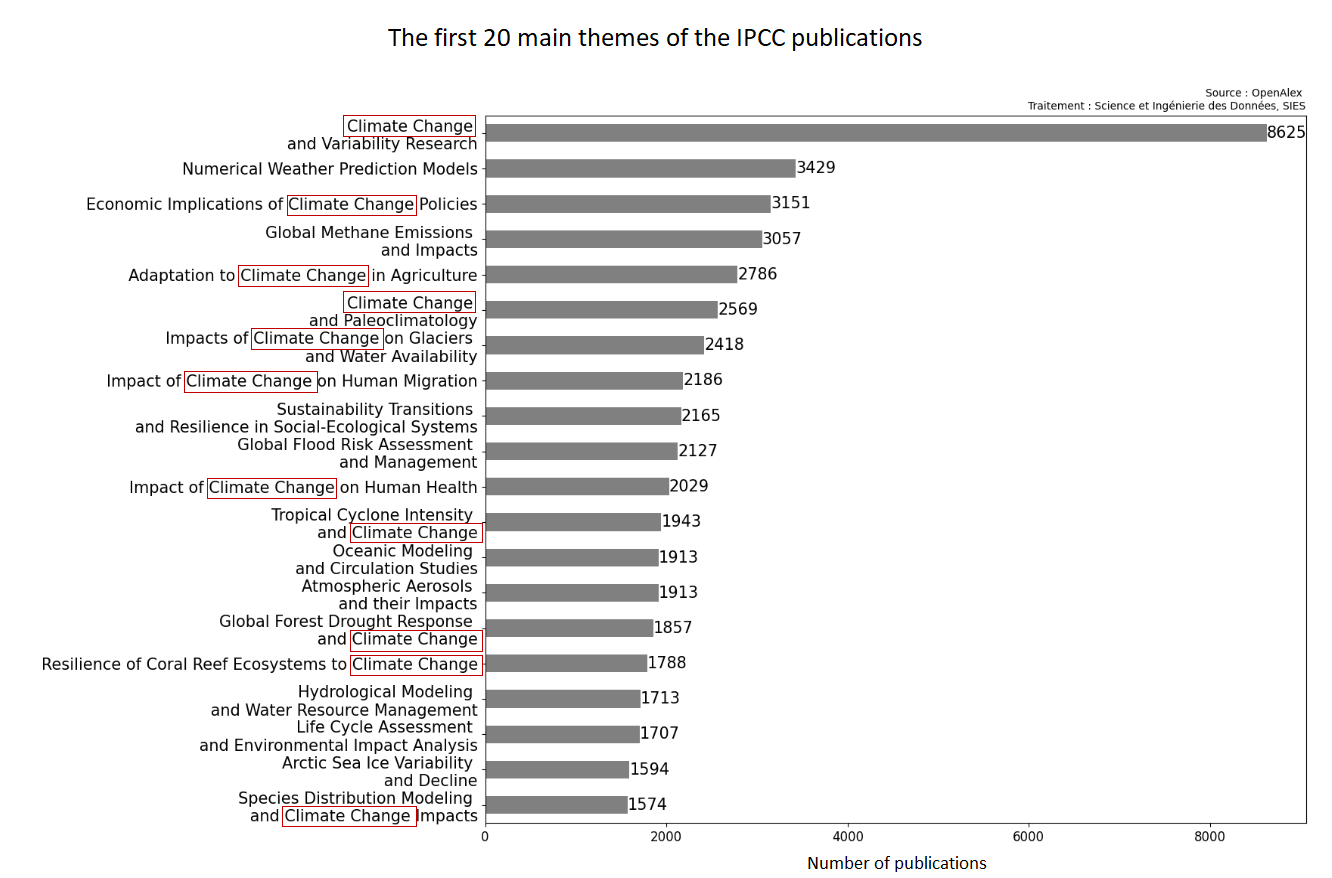
\includegraphics{./images/topics_distribution_IPCC_model_fr.png}
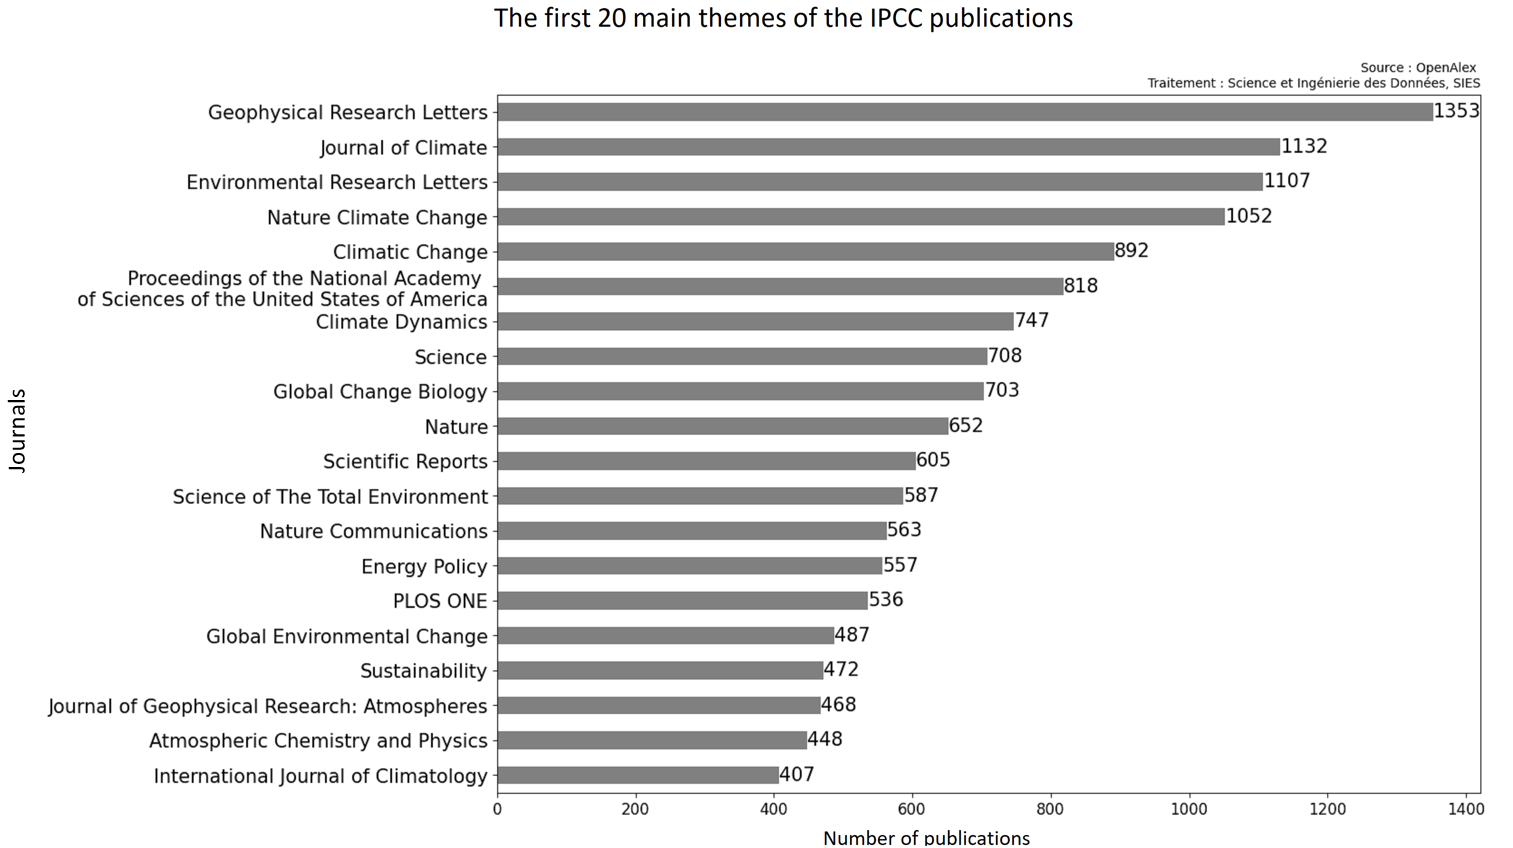
\includegraphics{./images/locations_distribution_IPCC_model.png} We
conclued that the publications from the reports are recents, less than
10 years old for 90\% of them. Some keywords seems to appear frequently,
like ``Climate Change'' and many scientific journals release IPCC
publications.

Using the OpenAlex API, we found 48,219 publications that meet the
following criteria:

\begin{enumerate}
\def\labelenumi{\arabic{enumi}.}
\tightlist
\item
  Publications that are \textbf{not cited by the IPCC}.
\item
  Publications that \textbf{do not contain specific terms} according to
  the top topics, such as ``climate change'' or ``environmental impact''
  in their topics, ensuring that our model remains unbiased.
\item
  Publications that have a \textbf{global temporal distribution
  equivalent} to the IPCC's cited publications. For example, in 2018,
  there were 6,755 publications cited by the IPCC, so we retrieve 6,755
  publications from OpenAlex that exclude certain themes. This process
  is repeated for each year in the temporal distribution of IPCC
  publications.
\end{enumerate}

We conduct the exact same method for the IPBES report.

\hypertarget{train-the-model}{%
\subsection{2.5 Train the model}\label{train-the-model}}

Once the dataset is complete, we split it in two:

\begin{itemize}
\tightlist
\item
  80\% of data will be used to train the model
\item
  20\% will be used as a test base
\end{itemize}

To train the model, we use fasttext. FastText is a library developed by
Facebook AI Research for learning word representations and text
classification. Unlike Word2Vec, FastText breaks words into subwords,
improving its ability to handle rare or out-of-vocabulary words. It's
fast, efficient, and supports multilingual models, making it ideal for
various natural language processing tasks like sentiment analysis and
text classification.

Fasttext enable to vectorize and apply a linear regression on the data

\hypertarget{results}{%
\section{3. Results}\label{results}}

\hypertarget{graphs-of-ipcc-bibliography-analysis}{%
\subsection{3.1 Graphs of IPCC bibliography
analysis}\label{graphs-of-ipcc-bibliography-analysis}}

\hypertarget{custom-perimeter}{%
\subsection{3.2 Custom perimeter}\label{custom-perimeter}}

\hypertarget{code-availibility}{%
\section{4. Code availibility}\label{code-availibility}}

The code developed is open source and available online on GitHub
\url{https://github.com/dataesr/teds}

\hypertarget{references}{%
\section*{References}\label{references}}
\addcontentsline{toc}{section}{References}

\hypertarget{refs}{}
\begin{cslreferences}
\leavevmode\hypertarget{ref-10.1162ux2fqss_a_00179}{}%
Chaignon, Lauranne, and Daniel Egret. 2022. ``Identifying Scientific
Publications Countrywide and Measuring Their Open Access: The Case of
the French Open Science Barometer (Bso).'' \emph{Quantitative Science
Studies} 3 (1): 18--36. \url{https://doi.org/10.1162/qss_a_00179}.

\leavevmode\hypertarget{ref-ipccbibliography}{}%
n.d.a. \url{https://www.ipcc.ch/report/ar6}.

\leavevmode\hypertarget{ref-ipbesbibliography}{}%
n.d.b.
\url{https://www.zotero.org/groups/2333077/ipbes_global_assessment/library}.
\end{cslreferences}


\end{document}
